\documentclass[a4paper,12pt,pdftex]{article}

\usepackage{fancyhdr}
\usepackage{parskip}
\usepackage[utf8]{inputenc}
\usepackage{hyperref}
\usepackage{listings}
\usepackage{graphicx}
\newcommand{\HRule}{\rule{\linewidth}{0.2mm}}

\def\name{Ole Henrik Paulsen}
\def\studentnumber{130572}
\def\course{Machine Learning and Pattern Recognition | IMT4612}
\def\school{Gjøvik University Collage}
\def\reportname{Assigment 2}
% Spring, 2013 - Autumn, 2010 - Both are valid
\def\semester{Spring 2014}

\hypersetup
{
    pdftitle={\reportname},
    pdfauthor={\name},
    pdfsubject={\reportname},
    colorlinks=true,
    linkcolor=blue,
    citecolor=blue,
    urlcolor=blue   
}

\fancypagestyle{titlefooter}
{                                                                               
    \fancyhf{}                                                                  
    \fancyfoot[c]{\footnotesize This document was compiled on \today}           
} 

\begin{document}

\begin{titlepage}                                                               
    \begin{center}                                                                                                   
                                                                                
        \large \course\\                                                        
        \large \school, \semester\\[0.4cm]                                       
        \HRule\\[1.5cm]                                                         
                                                                                
        \begin{minipage}{0.4\textwidth}                                         
            \begin{flushleft}                                                   
                % Some lecturers does not want to know your name...
                \small \emph{Author:} \name\\                                  
                \small \emph{Student number:} \studentnumber\\                  
            \end{flushleft}                                                     
        \end{minipage}                                                          
                                                                                
        \ \\[7.0cm]                                                             
        \LARGE\textbf{\reportname}                                              
                                                                                
    \end{center}                                                                
    \thispagestyle{titlefooter}                                                 
\end{titlepage}                                                                 
                                                                                
\tableofcontents                                                                
\clearpage   

\begin{abstract}

    Assigment 2 in Machinelearning

\end{abstract}

\section{Learning as a Search}
\subsection{Global optimal solutions}

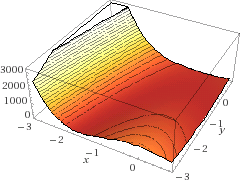
\includegraphics{3dplot.png}

The global minima in the fitness function are (-1,-1) 

This can be calculated with this equaction:

min(75(y + x**2)**2 + (1 +x)**2) = 0

\subsection{Genetic Algorithm(GA)}

This section is done in Python with the library Numpy for max, min and array
handling(matrix). 

I made a Class that takes alot of variables that you easy can edit to optimize
the genetic algorithm. 

The seed is made of random numbers between two values. random(-10,10) will give
you a random number from -10 to 10. 

The selection function are selecting the 4 best chromosomes and deleting the
rest of the set. 

Crossover are switching randomly x-values or y-values from a perrent with an
other perrent. The new pair are added to the set for next generation.

There is also spawning a new random pair of (X,Y) evry generation. The only
ruule for this new random spawned pair is that is not alleready in the set of
cromosomes. 

The fitnes function is takeing a X and Y value as input and returing the number
of the equation. 

When the final generation of rouds are done it hopyfully retturing the cords
-1,-1.



\subsection{Gradient Descent method}
\subsection{Performance domain}

\section{Statistical Learning}
\subsection{Computer program}
I did the programming in Python with the library Numpy and Time. You need to install Numpy, but time is a core
library of Python. Numpy are used to handle sqrt, max, min and mathematical functions on arrays. I also used Numpy
to read in data from the txt files. Numpy also have functions for Euclidean and chebyshev, but they are NOT used in my program.

K Neaarest Neighbor are also programmed by from the bottom instead of using a library. 

*K nearst Neighbor code*

The program are scaled to handle large amount of input, both train and validation data, and 13 attributes takes under 3 secounds to handle.

\subsection{Read input files}

The train.txt and validation.txt are read into the program with Numpy's genfromtxt.
*genfromtxt code* 

I save the input data in a masked arrays. and split out the label into a own array.

*Splitting code* 

I confirm the input is 120 train samples and 10 validation samples in the output.

\subsection{Radar and Area plot}
I built the graphs under in Excel afterr hours of trying and failing in
matplotlib and numpy. 

Some of the graphs are using logarithmcs scala on the axis. 

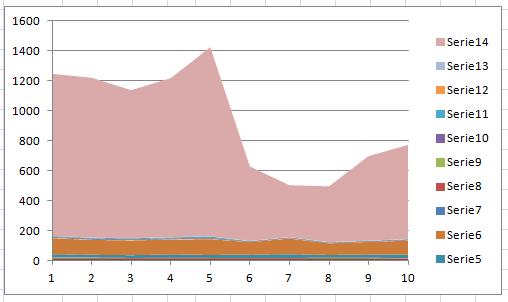
\includegraphics{stackplot.png}

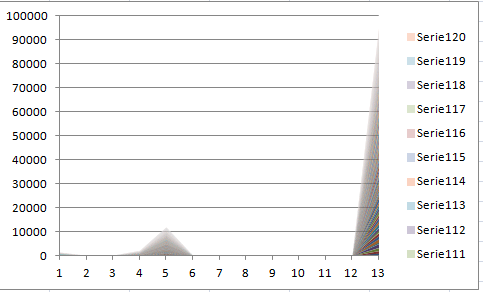
\includegraphics{stackplot2.png}

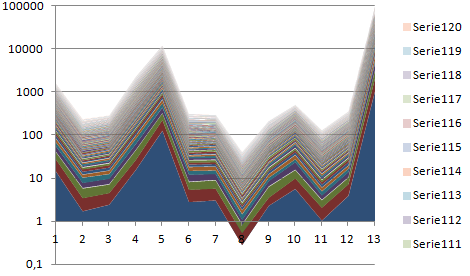
\includegraphics{stackplot3.png}

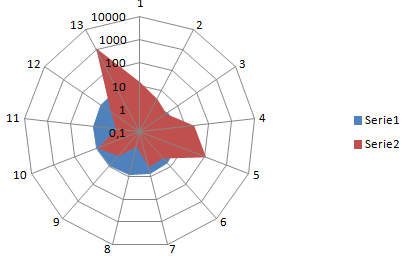
\includegraphics{radarplot.png}

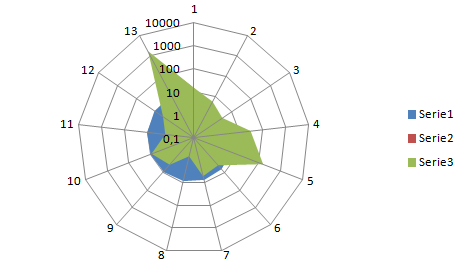
\includegraphics{radar2.png}

*

\subsection{Distance Algorythms}

The follow three algorithms are included into the program:

Euclidean:

Squar Euclidean:

Chebyshev:

As you can see they got different output from each other
\subsection{Output}

The output of the program is as follow:

*Output from the program*

\nocite{*}

\bibliographystyle{acm}
\bibliography{references}

\end{document}
